\newpage
\section{Three-dimensional single fin}
\label{chapter-3Dsinglefin}
%
This test case investigates the Mach 4 air flow over a three-dimensional flat plate with $16^{\circ}$ angled fin, based on the experimental and computational analysis of an identical geometry by Kim et. al.~\cite{kim1991}. 

The experiments by Kim~\cite{kim1991} involved measuring skin friction coefficient $C_f$ and pressure along an arc $\beta$ of constant radius ($88.9$\,mm) over the flat plate surface, centred about the fin's leading edge. Flows at Mach 3 and 4, and fin angles $\alpha$ of $10^{\circ}$, $16^{\circ}$ and $20^{\circ}$ were tested.

Numerous tests featuring this fin and flat plate geometry (due to the use of the same experimental facility) have been completed and recorded in a database~\cite{settles1991} for validation purposes, including a series of measurements by Lu~\cite{lu1988} for the incoming flat plate boundary layer, and a similar simulation by Panaras~\cite{panaras97}. This data provides sufficient information to properly validate the results of the Eilmer3 simulation.
 
%------------------------------------------------------------------
\subsection{Details of flow problem}
%\label{}
Figure~\ref{f:tc2:scheme} indicates the basic flow schematic for the test case. 
The schematic features a $0.216$\,m flat plate `run-up', after which the flow is deflected by a $127$\,mm$\times76$\,mm fin angled ($\alpha$) $16^{\circ}$ to the incoming flow. The flow across the `run-up' flat plate will result in the formation of a weak oblique shock and turbulent boundary layer. The second oblique shock that develops from the flow interaction with the fin is expected to cause flow separation close to the fin-plate interface, due to interaction with the incoming turbulent boundary layer.
%
\begin{figure}[htbp]
 \begin{center}
  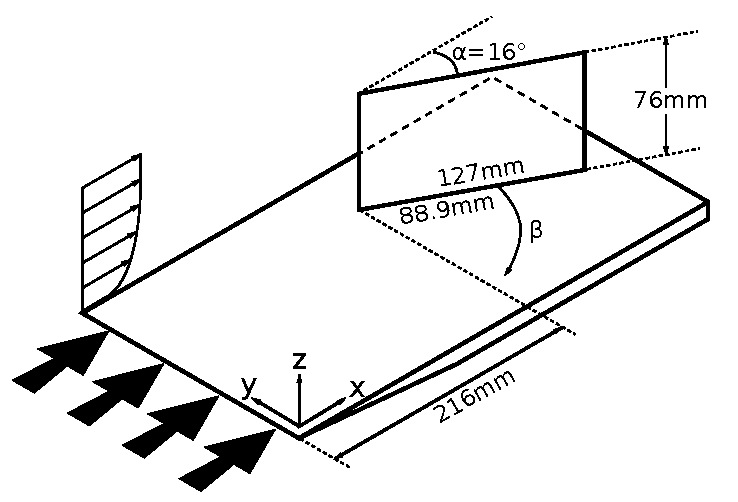
\includegraphics[width=9cm]{./chap7-3Dsinglefin/figs/schematic2annotated2.pdf}
  \caption{Basic Schematic for Single Fin Simulation (not to scale).}
  \label{f:tc2:scheme}
 \end{center}
\end{figure}
%

A Mach number of 4 was selected to replicate a validated flow field and test arrangement by Kim~\cite{kim1991}. Test conditions for the associated experiment were supplied as indicated in Table~\ref{t:tc2:supplied}. Compressible flow theory (Equation~\ref{e:comp1}-\ref{e:comp3}) was used to convert the conditions into fluid properties for use in the simulation (Table~\ref{t:tc2:initial}).
%
\begin{equation}
  \label{e:comp1}
  \frac{T_\infty}{T_0}=\left(1+\frac{\gamma-1}{2}M^2\right) \,\,\,\,\,\,\,\,\,\,\,\,\,\,\,\,\,\,\,\, \frac{P_\infty}{P_0}=\left(1+\frac{\gamma-1}{2}M^2\right)^\frac{\gamma}{\gamma-1}
\end{equation}
\begin{equation}
  \label{e:comp3}
  Re=\frac{\rho U_\infty}{\mu} \,\,\,\,\,\,\,\,\,\,\,\,\,\,\,\,\,\,\,\, M = \frac{U_\infty}{\sqrt{\gamma R T_\infty}} = \frac{U_\infty}{\sqrt{\frac{\gamma P_\infty}{\rho}}}
\end{equation}


\begin{table}[htbp]
  
  \caption{3D Single Fin Test Conditions.}
  \label{t:tc2:supplied}
  \begin{center}
  \begin{tabular}{cccl}
  \hline\hline
     Property  & Value & Units \\
  \hline
    $M$  & $4$ $(3.98)$ & \\
    $P_0$  & $1.524\times10^6$ & Pa  \\
    $T_0$  & $293.4$ & K  \\
    $Re$  & $6.79\times10^7$ & /m  \\
  \hline\hline
  \end{tabular}
  \end{center}
\end{table}
%
%
\begin{table}[htbp]
  
  \caption{3D Single Fin Initial \& Inflow (Freestream) Conditions.}
  \label{t:tc2:initial}
  \begin{center}
  \begin{tabular}{cccl}
  \hline\hline
     Property  & Value & Units \\
  \hline
    $P_\infty$  & $10300$ & Pa  \\
    $U_\infty$  & $707.0$ & m/s  \\
    $T_\infty$  & $70.4$ & K  \\
    $\rho_\infty$  & $0.457$ & kg/m$^3$  \\
  \hline\hline
  \end{tabular}
  \end{center}
\end{table}
%

The data supplied by Kim~\cite{kim1991} did not identify initial turbulence variables. A turbulence intensity of $1\%$ and turbulent-to-laminar viscosity ratio of $1$ were selected to initialise $k$ and $\omega$, as indicated in Table~\ref{t:tc2:turb}.
%
\begin{table}[htbp]
  
  \caption{3D Single Fin Initial (Freestream) Turbulence Properties.}
  \label{t:tc2:turb}
  \begin{center}
  \begin{tabular}{cccl}
  \hline\hline
     Property  & Value & Units \\
  \hline
    Turbulence Kinetic Energy ($k$)  & $74.98$ & m$^2$/s$^2$  \\
    Specific Dissipation Rate ($\omega$)  & $80.32\times10^5$ & /s  \\
  \hline\hline
  \end{tabular}
  \end{center}
\end{table}
%

\subsection{Details of computational approach}
%\label{}

Due to the large domain size of the flat plate and fin arrangement, the test case was split into two separate geometries to be simulated individually. The first geometry was a two-dimensional flat plate `run-up', representative of a 2D $x$-$z$ slice of the flat plate fluid domain. This domain was a $240$\,mm$\times27.69$\,mm rectangle divided into a $256\times111$ cell mesh, as indicated in Figure~\ref{f:tc2:runup}. The south face is represented as an adiabatic wall, with cells clustered towards the plate surface to ensure a $y^+<1$. The extra length allows for the turbulent boundary layer to fully develop, and for a data profile to be extracted at a desired length along the flat plate for use as inflow for the 3D simulation. 
%
\begin{figure}[htbp]
 \begin{center}
  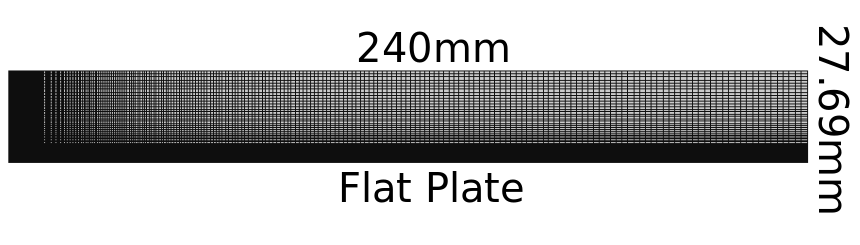
\includegraphics[width=12cm]{./chap7-3Dsinglefin/figs/tc2-runup.png}
  \caption{3D Single Fin `Run-up' Mesh.}
  \label{f:tc2:runup}
 \end{center}
\end{figure}
%

The second geometry was a three-dimensional, two-block arrangement featuring a $10$\,mm$\times99.8$\,mm$\times20$\,mm `run-up' block attached to a $86.5$\,mm$\times20$\,mm fin block with $Y$ reduction from $99.8$\,mm to $75$\,mm (Figure~\ref{f:tc2:coordinates}). The `run-up' block was included to allow flow development in 3D before interaction with the angled fin. A $99.8$\,mm width was selected, as this was sufficient to capture the oblique shock produced by the angled fin. Trigonometric relations were used to size the fin block after selecting a deflection angle $\alpha$ of $16^{\circ}$ and fin length of $90$\,mm. 

The fin length was reduced from the physical length of $127$\,mm, as the experimental data was extracted at a radius of $88.9$\,mm. Additionally, the height of the fin was reduced to $20$\,mm from $76$\,mm, as the turbulent vortex initiated at the leading edge of the fin and flat plate were found to not exceed this height~\cite{panaras97}. The reduced dimensions ensure the flow is fully developed at the data extraction region, while the fluid domain size and cell count is minimised. 
%
\begin{figure}[htbp]
 \begin{center}
  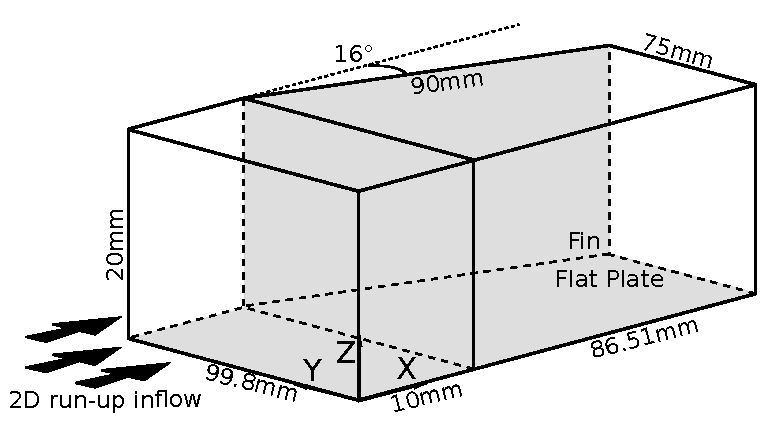
\includegraphics[width=14cm]{./chap7-3Dsinglefin/figs/3Dcoordinates2.pdf}
  \caption{3D Single Fin Mesh Geometry (not to scale).}
  \label{f:tc2:coordinates}
 \end{center}
\end{figure}
%

The flat plate and fin surfaces (shown in grey in Figure~\ref{f:tc2:coordinates}) were set to adiabatic walls to allow viscous effects and further development of the incoming turbulent boundary layer. The north boundary of the `run-up' was set to a slip wall, to encourage flow interaction with the fin leading edge. All other surfaces were set as open boundaries through the use of $ExtrapolateOutBC$. 

The 3D geometry was split into a $15\times100\times100$ `run-up' mesh and a $85\times100\times100$ fin mesh ($1000000$ cells total, Figure~\ref{f:tc2:mesh}). Cells were strongly clustered towards the flat plate (bottom boundaries) and fin (north boundaries) to ensure $y^+<1$, with weaker clustering towards the 3D `run-up' and fin block interface (Figure~\ref{f:tc2:mesh}). Compatibility with the 2D `run-up' data was ensured through the use of an inflow profile interpolator, allowing the higher-resolution 2D run-up data to be downscaled to the smaller 3D resolution. 
%
\begin{figure}[htbp]
 \begin{center}
  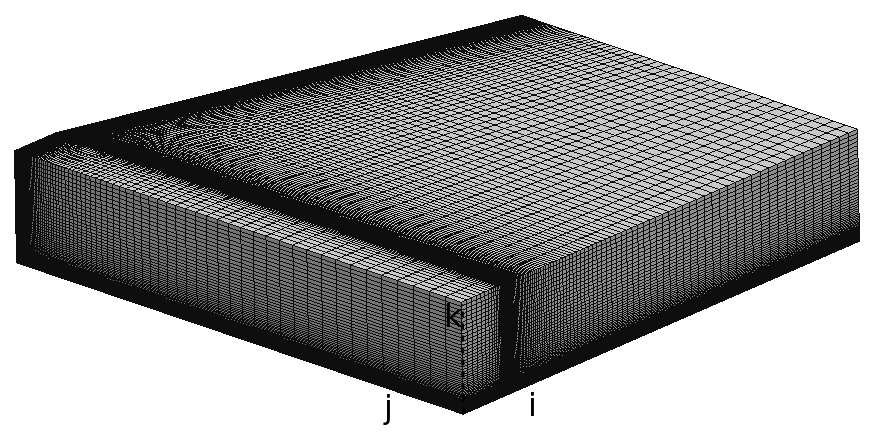
\includegraphics[width=12cm]{./chap7-3Dsinglefin/figs/tc2-mesh.png}
  \caption{3D Single Fin Simulation Mesh.}
  \label{f:tc2:mesh}
 \end{center}
\end{figure}
%

The two-dimensional `run-up' domain was split into $64$ blocks ($8\times8$), as was the three-dimensional domain ($4\times4\times4$), in an effort to minimise simulation time. The clustering of the cells in the $Z$ direction was identical, ensuring the 2D outflow profile correctly correlates with the cells in the 3D geometry.

\subsection{Results \& discussion}
%\label{}
\subsubsection{2D Single Fin `Run-up' Results}
%\label{}
%
The two-dimensional `run-up' was tested for $0.92$ milliseconds (approximately three flow lengths) in order to ensure the flow had reached steady state conditions. This required a `Barrine' simulation lasting $46.8$ hours ($2995.2$ CPU-hours). 

Figure~\ref{f:tc2:runupmach} indicates pressure over the `run-up' domain. As distance from the leading edge ($X$) increases, the boundary layer is observed to increase in thickness, as expected. An oblique shock, caused by the interaction with the flat plate leading edge, is also observable as the change in pressure and can be seen leaving the north boundary.
%
\begin{figure}[htbp]
 \begin{center}
  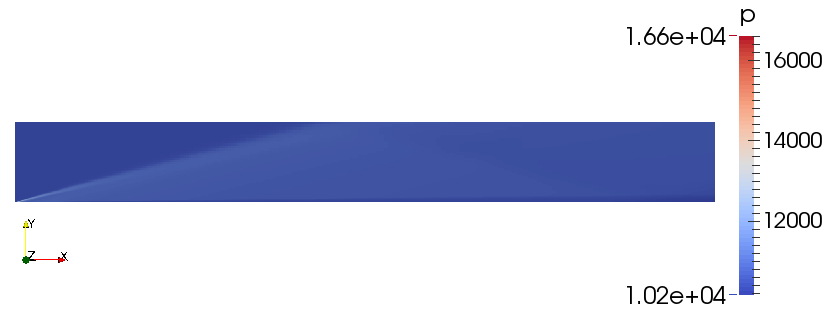
\includegraphics[width=14cm]{./chap7-3Dsinglefin/figs/tc2-runup-mach.png}
  \caption{2D Single Fin `Run-up' Pressure Data.}
  \label{f:tc2:runupmach}
 \end{center}
\end{figure}
%

The flow data at $x=0.206$\,m was interpolated to the lower 3D resolution and extrapolated into the third dimension, for use as inflow for the 3D simulation. This allows for the $10$\,mm of 3D `run-up' domain to further develop the turbulent boundary layer before it interacts with the fin, ensuring the total `run-up' of $216$\,mm is replicated.

\subsubsection{3D Single Fin Results}

While the two-dimensional run-up results were properly extracted and set as inflow for the 3D simulation, the checker-boarding phenomenon was found to still present (Figure~\ref{f:tc2:check1}). This was unexpected as, following the failure of the previous iterations, the cell-count was significantly increased and the flow domain was shortened in the Z direction. 
%
\begin{figure}[htbp]
 \begin{center}
  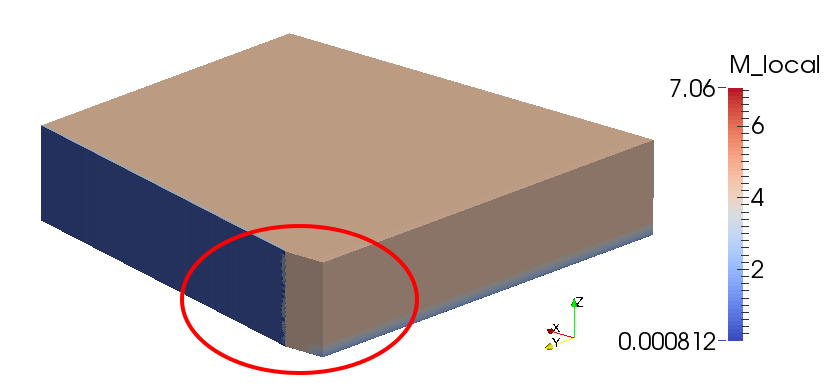
\includegraphics[width=12cm]{./chap7-3Dsinglefin/figs/tc2-mach1.png}
  \caption{3D Single Fin Mach Number Contours indicating checker-boarding.}
  \label{f:tc2:check1}
 \end{center}
\end{figure}
%
%
\begin{figure}[htbp]
 \begin{center}
  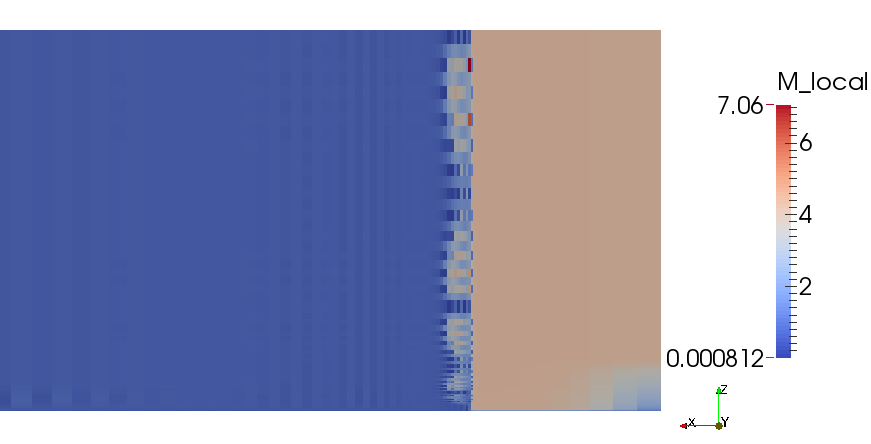
\includegraphics[width=12cm]{./chap7-3Dsinglefin/figs/tc2-mach2.png}
  \caption{3D Single Fin Mach Number Contours indicating checker-boarding on the leading edge of the fin.}
  \label{f:tc2:check2}
 \end{center}
\end{figure}
%

The checker-boarding appears on the leading edge of the fin (Figure~\ref{f:tc2:check2}), which results in simulation instability and abort after 5 microseconds of test time.  An avenue of future work for this test case would be to further investigate the cause of this phenomenon and prevent the onset of checker-boarding. 

Due to the strong clustering in the $Z$ direction, the $y^+$ criterion at the flat plate surface is much lower than $1$, however the cells at the upper boundary are stretched. By relaxing the clustering, but ensuring $y^+$ remains below $1$, the simulation may be less likely to become unstable. 

Alternatively, a small section of the domain containing the 3D `run-up' and the start of the fin could be simulated with a series of different clustering strengths and cell-counts, in order to investigate what conditions trigger the checker-boarding. This would allow the best cell structure to be selected and extrapolated into the full-size mesh, instead of repeatedly simulating full-size meshes that result in checker-boarding.